\documentclass[12pt]{article}
\usepackage[english]{babel}
\usepackage{natbib}
\usepackage{url}
\usepackage[utf8x]{inputenc}
\usepackage{amsmath}
\usepackage{graphicx}
\graphicspath{{images/}}
\usepackage{parskip}
\usepackage{fancyhdr}
\usepackage{subcaption}
\usepackage{relsize}
\usepackage{vmargin}
\setmarginsrb{3 cm}{2.5 cm}{3 cm}{2.5 cm}{1 cm}{1.5 cm}{1 cm}{1.5 cm}

\title{Statistical Pattern Recognition}								% Title
\author{94131091}								% Author
\date{\today}											% Date

\makeatletter
\let\thetitle\@title
\let\theauthor\@author
\let\thedate\@date
\makeatother

\pagestyle{fancy}
\fancyhf{}
\rhead{\theauthor}
\lhead{\thetitle}
\cfoot{\thepage}

\newcommand\numberthis{\addtocounter{equation}{1}\tag{\theequation}}
\newcommand{\gl}{^{>^{w_1}}_{<_{w_2}}}
\newcommand{\svector}[2]{\left[ \begin{matrix} #1 \\ #2 \end{matrix}\right]}
\newcommand{\smatrix}[4]{\left[ \begin{matrix} #1 & #2 \\ #3 & #4 \end{matrix}\right]}
\newcommand{\Pin}{\Pi_{i=1}^n}
\newcommand{\Sumn}{\Sigma_{i=1}^n}
\begin{document}

%%%%%%%%%%%%%%%%%%%%%%%%%%%%%%%%%%%%%%%%%%%%%%%%%%%%%%%%%%%%%%%%%%%%%%%%%%%%%%%%%%%%%%%%%

\begin{titlepage}
	\centering
    \vspace*{0.5 cm}
    
\includegraphics[scale = 0.8]{Imgs/logo.png}\\[1.0 cm]	% University Logo
    \textsc{\Large Computer Engineering \&\& IT Department\newline\newline Amirkabir University of Technology}\\[2.0 cm]	% University Name
%	\textsc{\large SPR\#1}\\[0.5 cm]				% Course Code
	\rule{\linewidth}{0.2 mm} \\[0.4 cm]
	{ \huge \bfseries \thetitle}\\
	\rule{\linewidth}{0.2 mm} \\[1.5 cm]
	
	\begin{minipage}{0.4\textwidth}
		\begin{flushleft} \large
			\emph{Submitted To:}\\
			Mohammad Rahmati\\
            Assoc. Professor\\
            Computer Engineering Department\\
			\end{flushleft}
			\end{minipage}~
			\begin{minipage}{0.4\textwidth}
            
			\begin{flushright} \large
			\emph{Submitted By :} \\
			Ahmad Asadi\\
            94131091\\
            Group-G1\\
            Fall-95\\
		\end{flushright}
        
	\end{minipage}\\[2 cm]
	
	
    
    
    
    
	
\end{titlepage}

%%%%%%%%%%%%%%%%%%%%%%%%%%%%%%%%%%%%%%%%%%%%%%%%%%%%%%%%%%%%%%%%%%%%%%%%%%%%%%%%%%%%%%%%%

\tableofcontents
\pagebreak

%%%%%%%%%%%%%%%%%%%%%%%%%%%%%%%%%%%%%%%%%%%%%%%%%%%%%%%%%%%%%%%%%%%%%%%%%%%%%%%%%%%%%%%%%
\section{Plotting conditional Parzen window based density estimates}
In the Parzen window formula, variable $V$ denotes the hypercube volume which given $h = 1$ is equal to 1. So the final formula is rewritten as \eqref{eq:1-1} in which $\omega_i$ denotes the $i$th class.
\begin{equation}
\hat{p}(x|\omega_i) = \frac{1}{n}\mathlarger{\Sigma}_{j=1}^{n_i} \phi(x - x_j)
\label{eq:1-1}
\end{equation}
According to \eqref{eq:1-1}, the first class conditional density estimate of first class based on Parzen window is expressed in \eqref{eq:1-2}.
\begin{equation}
\hat{p}(x|\omega_1) = \frac{1}{5}(\phi(x - x_1) + \phi(x - x_2) + \phi(x - x_3)) =  \frac{1}{5}(\phi(x - 4) + \phi(x - 1) + \phi(x - 5))
\label{eq:1-2}
\end{equation}
And that of the second class is expressed in \eqref{eq:1-3}.
\begin{equation}
\hat{p}(x|\omega_2) = \frac{1}{5}(\phi(x - x_4) + \phi(x - x_5)) =  \frac{1}{5}(\phi(x - 3) + \phi(x - 2))
\label{eq:1-3}
\end{equation}
Figure \ref{fig:1-1} displays both Parzen window estimated likelihood as a function of x for both classes.
\begin{figure}[h]
\centering
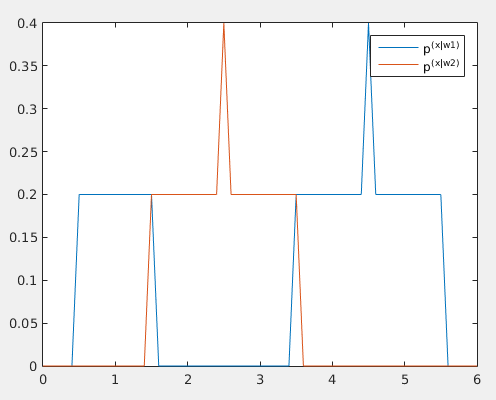
\includegraphics[scale=0.4]{Imgs/1-1.png}
\caption{Estimated likelihood of class conditional densities using Parzen window.}
\label{fig:1-1}
\end{figure}
%%%%%%%%%%%%%%%%%%%%%%%%%%%%%%%%%%%%%%%%%%%%%%%%%%%%%%%%%%%%%%%%%%%%%%%%%%%%%%%%%%%%%%%%%
\section{Plotting Parzen window estimate using Gaussian window function}
Equation \eqref{eq:2-1} represents the normal kernel.
\begin{equation}
\frac{1}{h^2}\phi(\frac{X-X_i}{h}) = (2\pi)^{-\frac{n}{2}}h^{-n}|\Sigma|^{\frac{1}{2}}exp[-\frac{1}{2}h^{-2}(X-X_i)^T\Sigma^{-1}(X-X_i)]
\label{eq:2-1}
\end{equation}
According to $\phi \sim N(0,1)$ the covariance matrix is $\Sigma = I$ and the mean vector is $\mu = 0$. The variable $n$ denoting the number of dimensions is equal to 2. So the normal kernel represented in \eqref{eq:2-1} is rewritten as equation \eqref{eq:2-2}.
\begin{equation}
\frac{1}{h^2}\phi(\frac{X-X_i}{h}) = (2\pi)^{-1}h^{-2}exp[-\frac{1}{2}h^{-2}(X-X_i)^T(X-X_i)]
\label{eq:2-2}
\end{equation}

The Parzen estimate is represented in \eqref{eq:2-3} in normal kernel case.
\begin{equation}
\hat{P} = \frac{1}{N}\mathlarger{\mathlarger{\Sigma}}_{i=1}^N \frac{1}{h^2}\phi(\frac{X-X_i}{h}) = \frac{1}{2N\pi h^2}\mathlarger{\mathlarger{\Sigma}}_{i=1}^Nexp[-\frac{1}{2}h^{-2}(X-X_i)^T(X-X_i)]
\label{eq:2-3}
\end{equation}

Using given dataset $x = \{<0.0, 1>; <0.1, 2>; <0.1, 9>; <0.3, 2>; <0.4, 1>; <0.4; 8>\}$ the Parzen estimate is computable. Figure \ref{fig:2-1} displays the estimated density using $h = 0.1$ and figure \ref{fig:2-2} displays estimated density in case of $h = 0.01$. 
\begin{figure}[h]
\centering
\begin{subfigure}{1\textwidth}
\centering
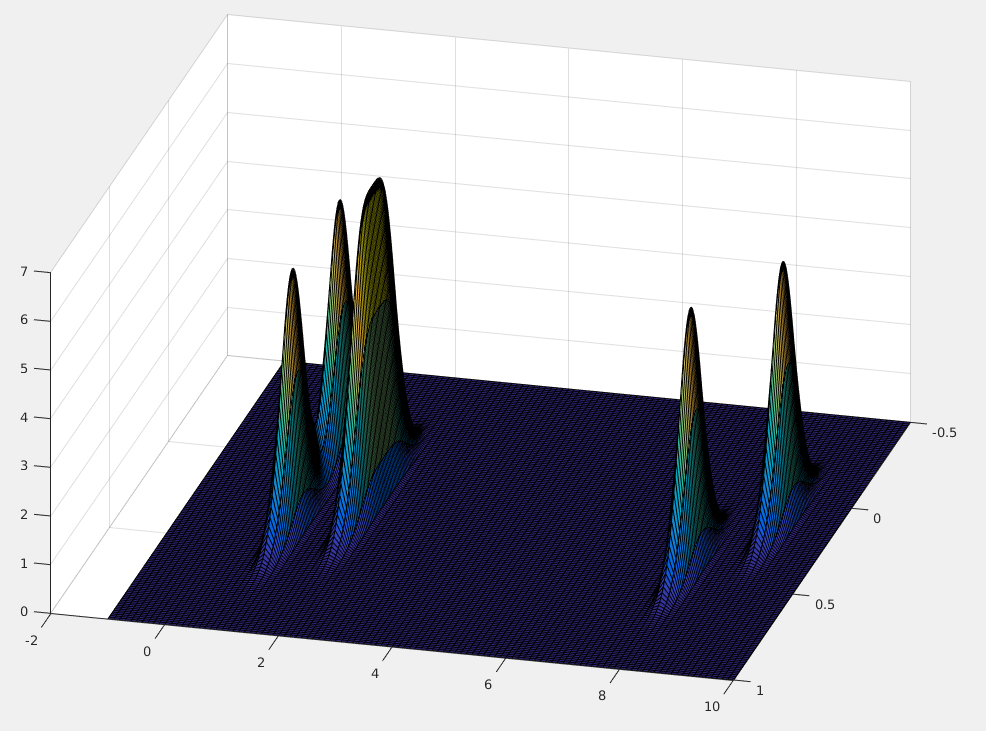
\includegraphics[scale=0.4]{Imgs/2-1.png}
\caption{Estimated density with $h = 0.1$}
\label{fig:2-1}
\end{subfigure}
\begin{subfigure}{1\textwidth}
\centering
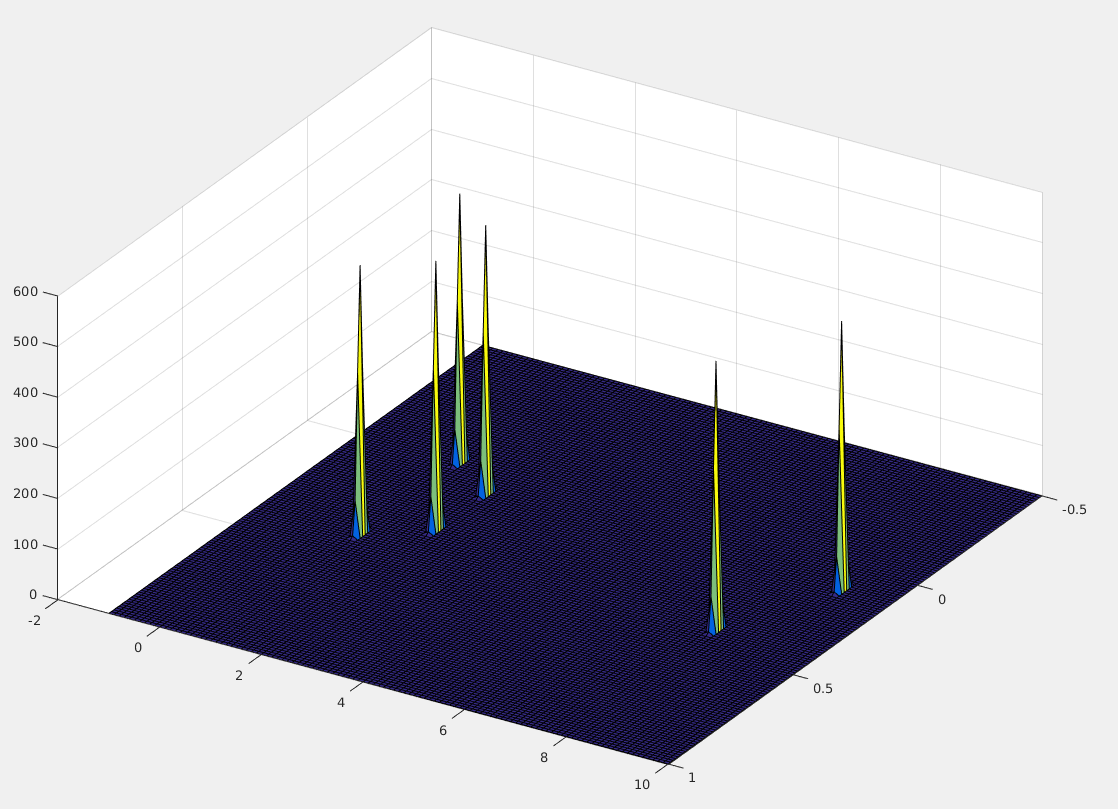
\includegraphics[scale=0.35]{Imgs/2-2.png}
\caption{Estimated density with $h = 0.01$}
\label{fig:2-2}
\end{subfigure}
\caption{Estimated density functions using Parzen Gaussian window}
\end{figure}

As it is clearly obvious, decreasing $h$ strongly makes model finer. The estimated density function is coarser when $h = 0.1$ rather than when $h = 0.01$.

\end{document}